%!TEX program = xelatex
\documentclass[10pt, compress]{beamer}
\usepackage[titleprogressbar]{../../cls/beamerthemem}

\usepackage{booktabs}
\usepackage[scale=2]{ccicons}
\usepackage{minted}

\usepgfplotslibrary{dateplot}

\usemintedstyle{trac}

\setbeamertemplate{caption}[numbered]
\setbeamertemplate{theorems}[numbered]
\newtheorem{crl}{Corollary}[theorem]
\newtheorem*{solution*}{Solution}

\usepackage{algorithm}
\usepackage[noend]{algpseudocode}

\usepackage{version}
%\excludeversion{proof}
%\excludeversion{solution*}

\usepackage{mathtools}
\usepackage{multicol}
\usepackage{qtree}

\makeatletter
\def\old@comma{,}
\catcode`\,=13
\def,{%
	\ifmmode%
	\old@comma\discretionary{}{}{}%
	\else%
	\old@comma%
	\fi%
}
\makeatother

\title{CSCI 3190 Tutorial of Week 11}
\subtitle{Longest Common Subsequence}
\author{LI Haocheng}
\institute{Department of Computer Science and Engineering}

\begin{document}

\maketitle

\begin{frame}[allowframebreaks]
	\frametitle{LCS between 3 Sequences}
	\begin{example}
		Consider the longest common subsequence problem between three sequences $A[1\cdots m]$, $B[1\cdots n]$ and $C[1\cdots p]$.
		Give a $O(mnp)$ dynamic programming based method to compute the longest common subsequence among
		these 3 sequences. 
	\end{example}

	\begin{algorithm}[H]
		\caption{Compute the LCS among 3 Sequences}
		\label{a-6}
		\begin{algorithmic}
			\Procedure{Three}{$A$, $B$, $C$}
			\State $T \coloneqq \Call{Zeros}{0 \cdots m, 0 \cdots n, 0 \cdots p}$
			\For{$j \coloneqq 1 \cdots m$} $T[j, 0, 0] \coloneqq 0$
			\EndFor
			\For{$k \coloneqq 1 \cdots n$} $T[0, k, 0] \coloneqq 0$
			\EndFor
			\For{$l \coloneqq 1 \cdots p$} $T[0, 0, l] \coloneqq 0$
			\EndFor
			\For{$j \coloneqq 1 \cdots m$}
			\For{$k \coloneqq 1 \cdots n$}
			\For{$l \coloneqq 1 \cdots l$}
			\If{$A[j] = B[k] = C[l]$} $T[j, k, l] \coloneqq T[j - 1, k - 1, l - 1] + 1$
			\Else\ $T[j, k, l] = \Call{Max}{T[j - 1, k, l], T[j, k - 1, l], T[j, k - 1, l]}$
			\EndIf
			\EndFor
			\EndFor
			\EndFor
			\State \Return $T[m, n, l]$
			\EndProcedure
		\end{algorithmic}
	\end{algorithm}
\end{frame}

\begin{frame}[allowframebreaks]
	\frametitle{Unique Symbols}
	\begin{example}
		Consider the longest common subsequence problem between sequence $A[1\cdots m]$ and sequence $B[1\cdots n]$ where
		the symbols in $A$ are all unique. Give a $O(n \log m)$ algorithm that can find the longest common subsequence
		between $A[1\cdots m]$ and $B[1\cdots n]$.
	\end{example}

	\textbf{Solution} Firstly use Algorithm \ref{a-7-1} to translate longest common subsequence problem to longest increasing subsequence problem. Secondly use Algorithm \ref{a-7-2} to solve it.
	\begin{algorithm}[H]
		\caption{Compute the LCS with Unique Symbols}
		\label{a-7-1}
		\begin{algorithmic}
			\Procedure{Translate}{$A$, $B$}
			\State $C \coloneqq \Call{Zeros}{n}$, $D \coloneqq \Call{Zeros}{{}}$
			\For{$j \coloneqq 1 \cdots m$} $D[A[j]] \coloneqq j$
			\EndFor
			\For{$k \coloneqq 1 \cdots n$} $C[k] = D[B[k]]$
			\EndFor
			\State \Return $C$, $D$
			\EndProcedure
		\end{algorithmic}
	\end{algorithm}
	\begin{algorithm}[H]
		\caption{Compute the LCS with Unique Symbols}
		\label{a-7-2}
		\begin{algorithmic}
			\Procedure{Unique}{$A$, $B$}
			\State $C, D \coloneqq \Call{Translate}{A, B}$
			\State $P \coloneqq \Call{Zeros}{n}$, $M \coloneqq \Call{Zeros}{n + 1}$, $l \coloneqq 0$
			\For{$k \coloneqq 1 \cdots n$}
			\State $lo \coloneqq 1$, $hi \coloneqq l$
			\While{$lo \le hi$}
			\State $mid \coloneqq \Call{Ceil}{\frac{lo + hi}{2}}$
			\If{$C[M[mid + 1]] < C[k]$} $lo \coloneqq mid + 1$
			\Else\ $hi \coloneqq mid - 1$
			\EndIf
			\EndWhile
			\State $P[k] = M[lo]$, $M[lo + 1] = k$
			\If{$lo > l$} $l = lo$
			\EndIf
			\EndFor
			\State $S \coloneqq \Call{Zeros}{l}$, $k = M[l + 1]$
			\For{$i \coloneqq l \cdots 1$} $S[i]=A[C[k]]$, $k = P[k]$
			\EndFor
			\State \Return $S$
			\EndProcedure
		\end{algorithmic}
	\end{algorithm}
\end{frame}

\begin{frame}[allowframebreaks]
	\frametitle{Tree}
	\begin{example}
		\begin{enumerate}[(a)]
			\item Show that the sum of the degrees of the vertices of a tree with $n$ vertices is $2n-2$.
			\item For $n \ge 2$, let $d_1, d_2, \cdots , d_n$ be $n$ positive integers such that $d_1 + d_2 + \cdots + d_n = 2n -2$. Show that there
			exists a tree whose vertices have degrees $d_1, d_2, \cdots, d_n$. 
		\end{enumerate}
	\end{example}
	\newpage
	\begin{proof}
		\begin{enumerate}[(a)]
			\item A $n$-vertex tree has $n-1$ edges so that the total degree is $2n - 2$.
			\item For $n = 2$, this is trivial. Suppose $\forall$ positive $d_i$ such that $\Sigma_{i = 1}^{n - 1} d_i = 2n - 4$, $\exists$ a tree $T^\prime$ whose vertices have degrees $d_1, d_2, \cdots, d_{n - 1}$. Then $\forall$ positive $d_i$ such that $\Sigma_{i = 1}^{n} d_i = 2n - 2$, since $d_i$ cannot be all greater than 1 or less than 2, without loss of generality, let $d_{n - 1} > 1, d_n = 1$. Hence we can remove $d_n$ and subtract $d_{n - 1}$ by 1 so that $\Sigma_{i = 1}^{n - 1} d_i = 2n - 4$ and we can find a tree $T^\prime$. After that we can add vertex $d_n$ as a leaf of $d_{n - 1}$ to build the final tree $T$.
		\end{enumerate}
	\end{proof}
\end{frame}

\begin{frame}[fragile]
	\frametitle{Traversal}
	\begin{columns}
		\begin{column}{.5\linewidth}
			\onslide<1->\begin{example}
				Construct a DFS and a BFS traversal for the graphs in Figure starting with node B as the root.
			\end{example}
			\onslide<2>\begin{solution*}
				\begin{enumerate}[(a)]
					\item \begin{description}
						\item[DFS] B, A, C, F, D, E
						\item[BFS] B, A, C, D, E, F
					\end{description}
					\item \begin{description}
						\item[DFS] B, A, D, E, C
						\item[BFS] B, A, C, D, E
					\end{description}
				\end{enumerate}
			\end{solution*}
		\end{column}
		\onslide<1->\begin{column}{.5\linewidth}
			\begin{figure}
				\centering
				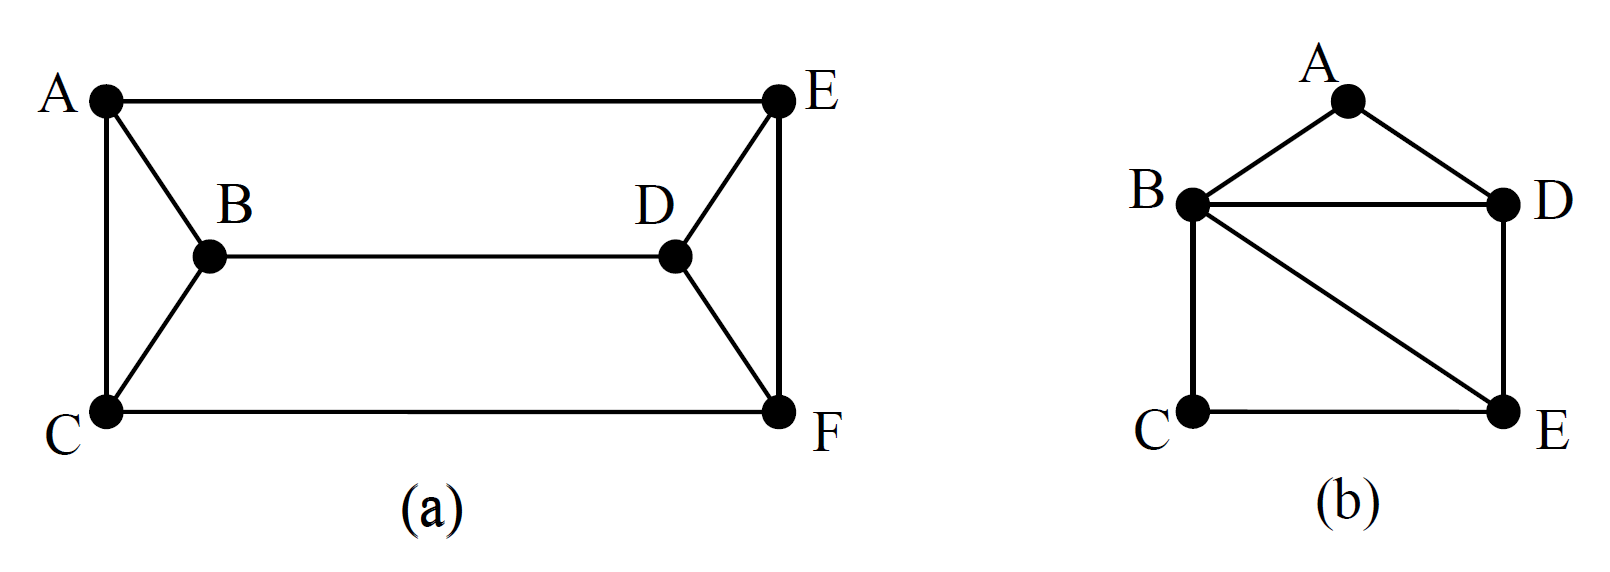
\includegraphics[width=\linewidth]{fg-1}
			\end{figure}
		\end{column}
	\end{columns}
\end{frame}

\plain{Questions?}

\end{document}
